%*******************************************************************************
%****************************** Second Chapter *********************************
%*******************************************************************************

\chapter{Overview of uncertainty modeling and propagation}
\label{cha:overview}

% **************************** Define Graphics Path **************************
\ifpdf
    \graphicspath{{Chapter2/Figs/Raster/}{Chapter2/Figs/PDF/}{Chapter2/Figs/}}
\else
    \graphicspath{{Chapter2/Figs/Vector/}{Chapter2/Figs/}}
\fi

% **************************** Chapter Abstract ******************************
\leftskip=1cm
\noindent
\emph{This chapter presents a brief overview of uncertainty modeling and structural reliability. It focuses on topics discussed in this dissertation from an engineering point of view. The main aim is to present the concepts, terms, notations, and methods used in further chapters. Emphasis is put on subjects that are typically insufficiently treated, overly simplified, or neglected in current civil engineering practice.}

\leftskip=0pt\rightskip=0pt


%****************************************************************************************
%****************************************************************************************
\section{Uncertainty modeling}

Statistical and interval based approaches are used to model and to propagate uncertainties. The former is used for most of the calculations, while interval analysis is only applied to represent measurement uncertainty and to compare with statistical approaches. Thus, interval analysis is introduced in the relevant chapter (Chapter~\ref{cha:error}). Since the mathematical machinery often appreciably differs from chapter to chapter, the particular, chapter-specific methods are introduced there. Here only the common, in multiple chapters utilized concepts are exposed.

The statistical analyses are completed using two main paradigms: frequentist and Bayesian statistics. The former views probability as a long-run frequency and bases inference on comparing the relative likelihood of datasets given a parameter value. Probability in the latter reflects the analyst's current state of knowledge using all available  information 
(``degree  of  belief''\footnote{It is often termed subjective probability; however, subjective here is not used in its everyday meaning. Instead it reflects the analyst's inevitable modeling assumptions and decisions, which are not solely based on the information conveyed by the data but on his or her expert judgment. Still the rationality and consistency are maintained: two analysts with the same experience and information would came up with the same inference.})
and  bases inference  on the relative evidence of the parameter values given a dataset \citep{Spiegelhalter2009, Cornell1970}. The latter is also regarded as the extension of classical logic \citep{Jaynes2003}.
It is out of the scope of this study to compare the frequentist and Bayesian paradigms in detail and to expose  the  deep  philosophical differences, see \citet{Jaynes2003, Barnett1999}. A brief comparison is presented in Table \ref{tab:freq_bay}, from which the most relevant for us are detailed in later sections. For a more comprehensive, practically oriented comparison see \citet{Wagenmakers2008, Jaynes1976}.
In later chapters mostly the Bayesian statistics is advocated and used due to that (\textit{i}) it represents all parameters with probability distribution thus enables the propagation and integration their uncertainty in further analysis, e.g. decision making; (\textit{ii}) allows to combine information from different sources; (\textit{iii}) and can efficiently handle complex problems with messy data.

The statistical techniques applied to estimate parameters, to construct uncertainty intervals, to account for distribution type uncertainty, to evaluate goodness-of-it, and to predict future observations are detailed in Annex~\ref{sec:stat_tools}. The descriptions are given in an extent to enable reproducibility.
The statistical techniques and notation used in further chapters are summarized in Table~\ref{tab:stat_methods_notations}.

% make the cells better looking!
\begin{table}
\caption{A brief comparison of frequentist and Bayesian statistics.}
\centering
\label{tab:freq_bay}
\small
\bgroup
\def\arraystretch{1.2}
    \begin{tabular}{m{0.24\textwidth} | m{0.35\textwidth} | m{0.35\textwidth}}
    \toprule
    Category & Frequentist  & Bayesian \\ 
    \midrule
    \rowcolor{lightgrey} Probability, $P$: & long-run frequency  &  degree of belief \\
    Parameters: & fixed but unknown &  random variables \\
    \rowcolor{lightgrey} Focuses on: & variability of data  &   uncertainty of knowledge \\
    Mathematical \newline machinery: & sampling distribution, repeated hypothetical experiments & Bayes' theorem, fixed data\\
    \rowcolor{lightgrey} Answers/calculates: & $P\left(\mathrm{data}|\mathrm{hypothesis}\right)$ &  $P\left(\mathrm{hypothesis}|\mathrm{data}\right)$ \\
    Source of information: & data (observations) &   data (observations) + prior belief \\
    \bottomrule
    \end{tabular}
\egroup
\end{table}



\mynote{not counting for cognitive differences and limitations (this latter problem is solved by Jaynes' robot)}
\mynote{note should be added that the term frequentist and bayesian a little vague, they should be understood with the given description and organization}



%\begin{landscape}
\begin{sidewaystable}[ht]
\caption{Summary of applied statistical methods and notations, for details see Annex~\ref{sec:stat_tools}.}
\centering
\label{tab:stat_methods_notations}
\small
	\begin{threeparttable}
    \begin{tabular}{lllll}
    \toprule
    Name\tnote{*} & Point estimate & \multicolumn{2}{l}{Uncertainty interval} & Model averaging \\
    \midrule
    Method of moments & MM  & -- & & -- \\
    \rowcolor{lightgrey}
    Generalized method of moments\tnote{\textdagger} & GMM  & delta & delta method\tnote{$\ddagger$} & -- \\ 
    \midrule
    \rowcolor{lightgrey}
    Maximum likelihood\tnote{\textdagger}  & ML  & delta & delta method & FMA (Eq.\ref{eq:FMA_point}-\ref{eq:FMA_var}) \\
    \rowcolor{lightgrey}
    ~ & ~  & proflike & profile likelihood  & ~ \\
    \rowcolor{lightgrey}
    ~ & ~  & bootstrap & bootstrapping  & ~  \\ 
    \midrule
    Bayesian posterior mean & BPM & hdi & highest density interval & BMA (Eq.\ref{eq:BMA}) \\
    ~ & ~ & eqi & equal tail interval & ~ \\
    Bayesian posterior predictive & BPP, (Eq.\ref{eq:postpred})& -- & & -- \\ 
    \bottomrule
    \end{tabular}
    \begin{tablenotes}
    \item[*] Examples for notation: \\
    ML-delta: maximum likelihood estimate with uncertainty interval constructed using delta method; \\
    BMA-BPM-hdi: Bayesian model averaged posterior mean estimate with highest density uncertainty interval.
    \item[\textdagger] \colorbox{lightgrey}{Frequentist paradigm.}
    \item[$\ddagger$] Similar to classic delta method but based on a special weighting matrix, see Section \ref{sec:interval_estimates}. 
    \item -- Not applicable/not available.
    \end{tablenotes}
    \end{threeparttable}
\end{sidewaystable}
%\end{landscape}

\mynote{summary, overview figure about treating parameter estimation and model selection uncertainty, might be better in Chapter 3}

%******************************************************************************************
%******************************************************************************************
\section{Structural reliability}
Structural reliability is concerned with the probabilistic analysis of engineering structures; most often this means the calculation of the failure probability of a structure with uncertain properties and subjected to uncertain actions. This problem is formulated using the limit state concept, which states that the boundary between safe and failure domain is sharp: characterized by a sudden change in performance. Accordingly, the related function is termed as performance function, $g(\mathbf{X})$. The limit state, $g(\mathbf{X})=0$, separates the disjoint safe and failure regions (Fig. \ref{fig:joint_dens}). The failure probability can be calculated as the integral of the joint density function of the random variables over the failure domain\footnote{This simple formulation is given for clarity, a more general formulation would include time, more general probabilistic models, and systems as well.}:
\begin{equation}
	\label{eq:Pf_general}
	 %{P_{\mathrm{f}}} = P\left( {g\left( {\bf{X}} \right) < 0} \right) = \int\limits_{g\left( {\bf{X}} \right) < 0} {{f_{\bf{X}}}({\bf{x}}) \cdot \mathrm{d}{\bf{x}}}.
	 {P_{\mathrm{f}}} = P\left( {g\left( {\bf{X}} \right) < 0} \right) = \int\limits_{g\left( {\bf{X}} \right) < 0} {p({\bf{x}}) \cdot \mathrm{d}{\bf{x}}}
\end{equation}
where $p(.)$ represents a probability density function that is identified by its argument. For example $p(x)$ and $p(y)$ are in general completely different functions. This notation allows greater clarity and conciseness than in reliability engineering typically used notation, $p(x) \equiv f_X(x)$.

The two main challenges in structural reliability are the inference of probabilistic models in the face of information scarcity, and the calculation of the typically high-dimensional integral (Eq.\ref{eq:Pf_general}). The integral is usually approximated by numerical techniques tailored for the particular features of structural reliability problems. These aim to reduce the required number of performance state function evaluations to minimal.

In this thesis, unless otherwise stated, the first order reliability method (FORM) \citep{Hasofer1974} is used for approximating the integral. It is sufficiently accurate for most structural engineering problems \citep{EN0}, though the presented calculations are often verified by more accurate methods, such as second order reliability method (SORM), Monte Carlo simulation (MC), and importance sampling Monte Carlo simulation (isMC).

The improved Hasofer-Lind-Rackwitz-Fiessler algorithm \citep{Rackwitz1979, Zhang1995} is used to solve the constrained optimization problem in FORM. For correlated random variables -- unless otherwise stated -- the Nataf transformation \citep{Liu1986} with Cholesky decomposition is used to obtain independent, normally distributed random variables. The asymptotic formula of \citet{Breitung1984} is used as a correction term in SORM. For isMC multivariate normal distribution used.

\begin{figure}[htbp!] 
	\centering    
	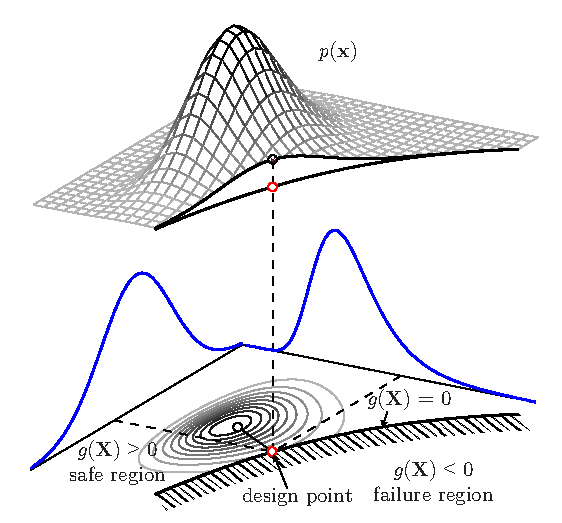
\includegraphics[width=0.6\textwidth]{joint_dens_illustration_fine_db.pdf}
	\caption{Illustration of limit state function, failure and safe regions, and design point.}
	\label{fig:joint_dens}
\end{figure}